\documentclass[xcolor=dvipsnames]{beamer}

\usepackage[utf8]{inputenc}
\usepackage{booktabs, subfig, graphicx, multirow}
\usepackage{tikz}
\usepackage[absolute,overlay]{textpos} 
\usetheme{PaloAlto}
\definecolor{TarletonPurple}{RGB}{79, 45, 127}
\usecolortheme[named=TarletonPurple]{structure}
\newenvironment{reference}[2]{
\begin{textblock*}{\textwidth}(#1,#2)              
  \footnotesize\it\bgroup\color{red!50!black}}{\egroup\end{textblock*}}


\graphicspath{{./Images/}}
%\setbeamercolor{frametitle}{bg=RoyalPurple}
%\setbeamercolor{sidebar}{bg=RoyalPurple}
%\setbeamercolor{logo}{bg=RoyalPurple!70!black!}



%% TITLE PAGE INFO%%
\title{Predicting Party Affiliation Using Social Media}
\author{Joseph Brown, Mikaela Jordan, and Adam Swayze}
\institute{Tarleton State University}
\date{April 1, 2016}

\begin{document}
\makeatletter
\def\beamer@framenotesbegin{
\begin{reference}{1mm}{1mm}
\tikz\node[opacity=0.8]{
\includegraphics[scale=0.25]{images/Tarleton_State_University}};
\end{reference} 

}
\makeatother
\frame{\titlepage}



%\begin{frame}
%\frametitle{Overview \hfill 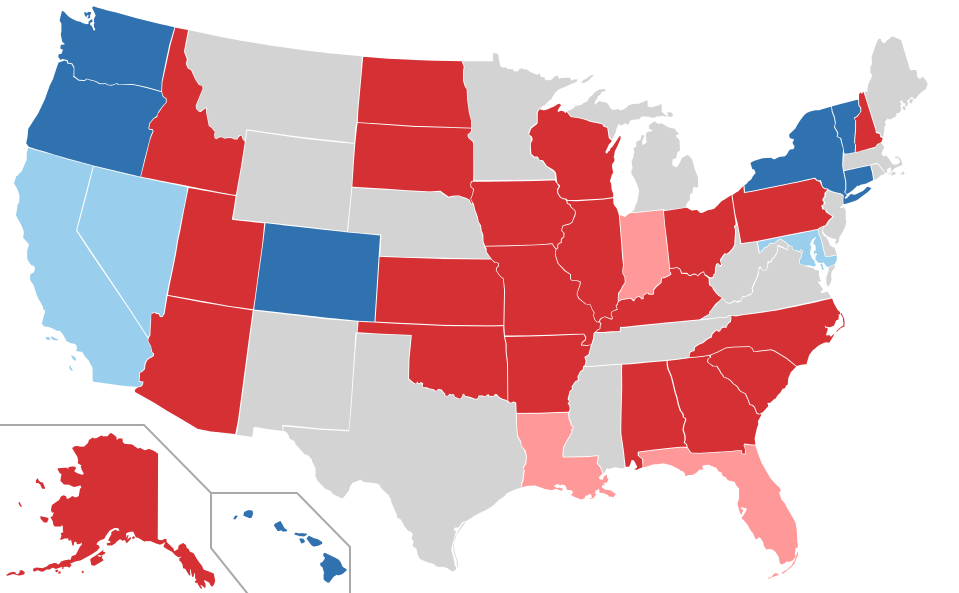
\includegraphics[scale=.04]{map.png}}
%
%\begin{itemize}
%\item Predicting Primary Results
%\begin{itemize}
%\item Use Twitter data to create a model that predicts primary results for each county.
%\end{itemize}
%\end{itemize}
%\end{frame}

\begin{frame}
\frametitle{Predicting Primary Results \hfill 
\includegraphics[scale=.15]{images/fivethirtyeight-logo}}

\begin{itemize}
\item In Primaries, polls change fast and are inaccurate	
\end{itemize}


\begin{figure}
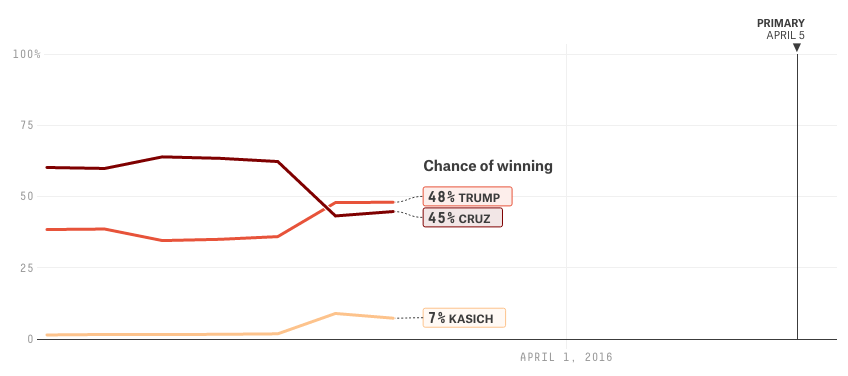
\includegraphics[scale=.35]{poll2.png}
\caption{Current polls for the Wisconsin Republican Primary from 538}
\end{figure}

\end{frame}


\begin{frame}
\frametitle{Alternative Primary Predictions \hfill 
\includegraphics[scale=.035]{images/facebook.png}}
\section{Polling and Predictions}
\begin{itemize}
\item Counties colored by Candidate with most Facebook likes 
\end{itemize}
\begin{center}

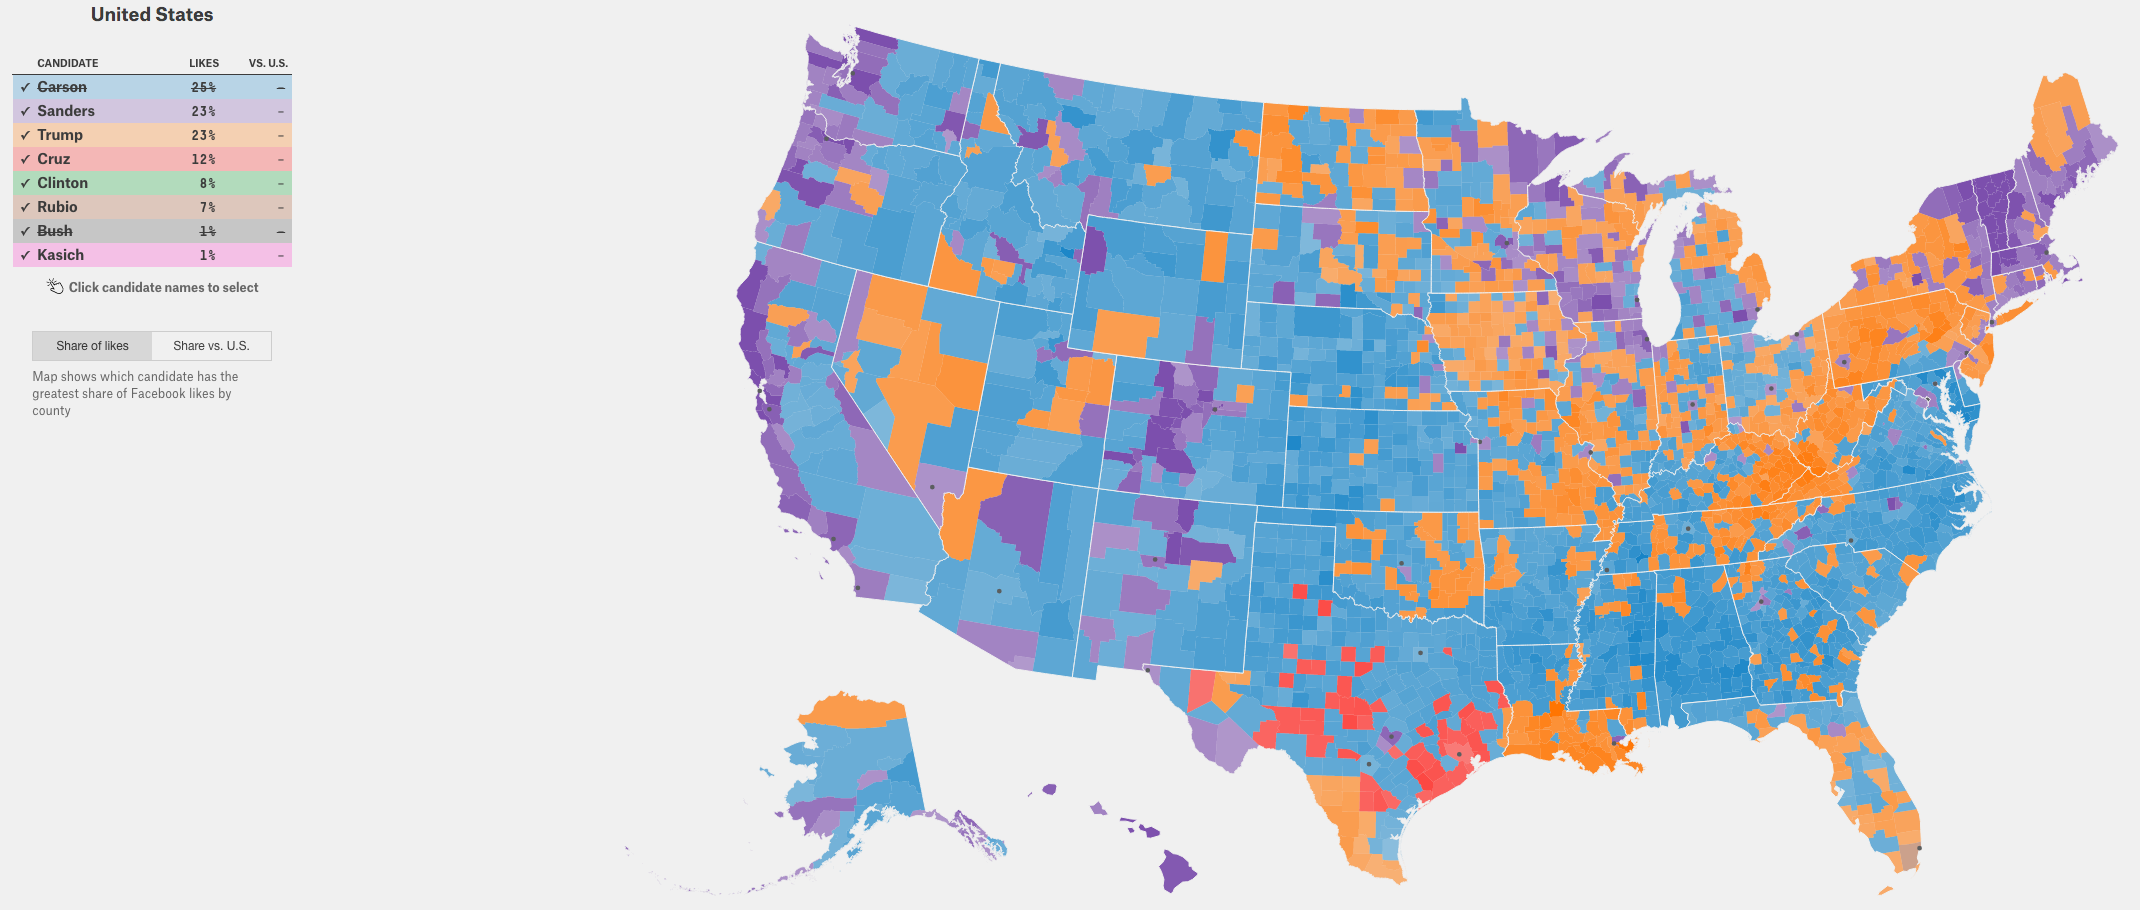
\includegraphics[scale=.14]{allmap.png}
\end{center}
\end{frame}

\begin{frame}
\frametitle{Candidates and Social Media  \hfill 
\includegraphics[scale=.015]{images/likes.png}}

\begin{itemize}
\item Candidates still running for President
\end{itemize}
\begin{center}

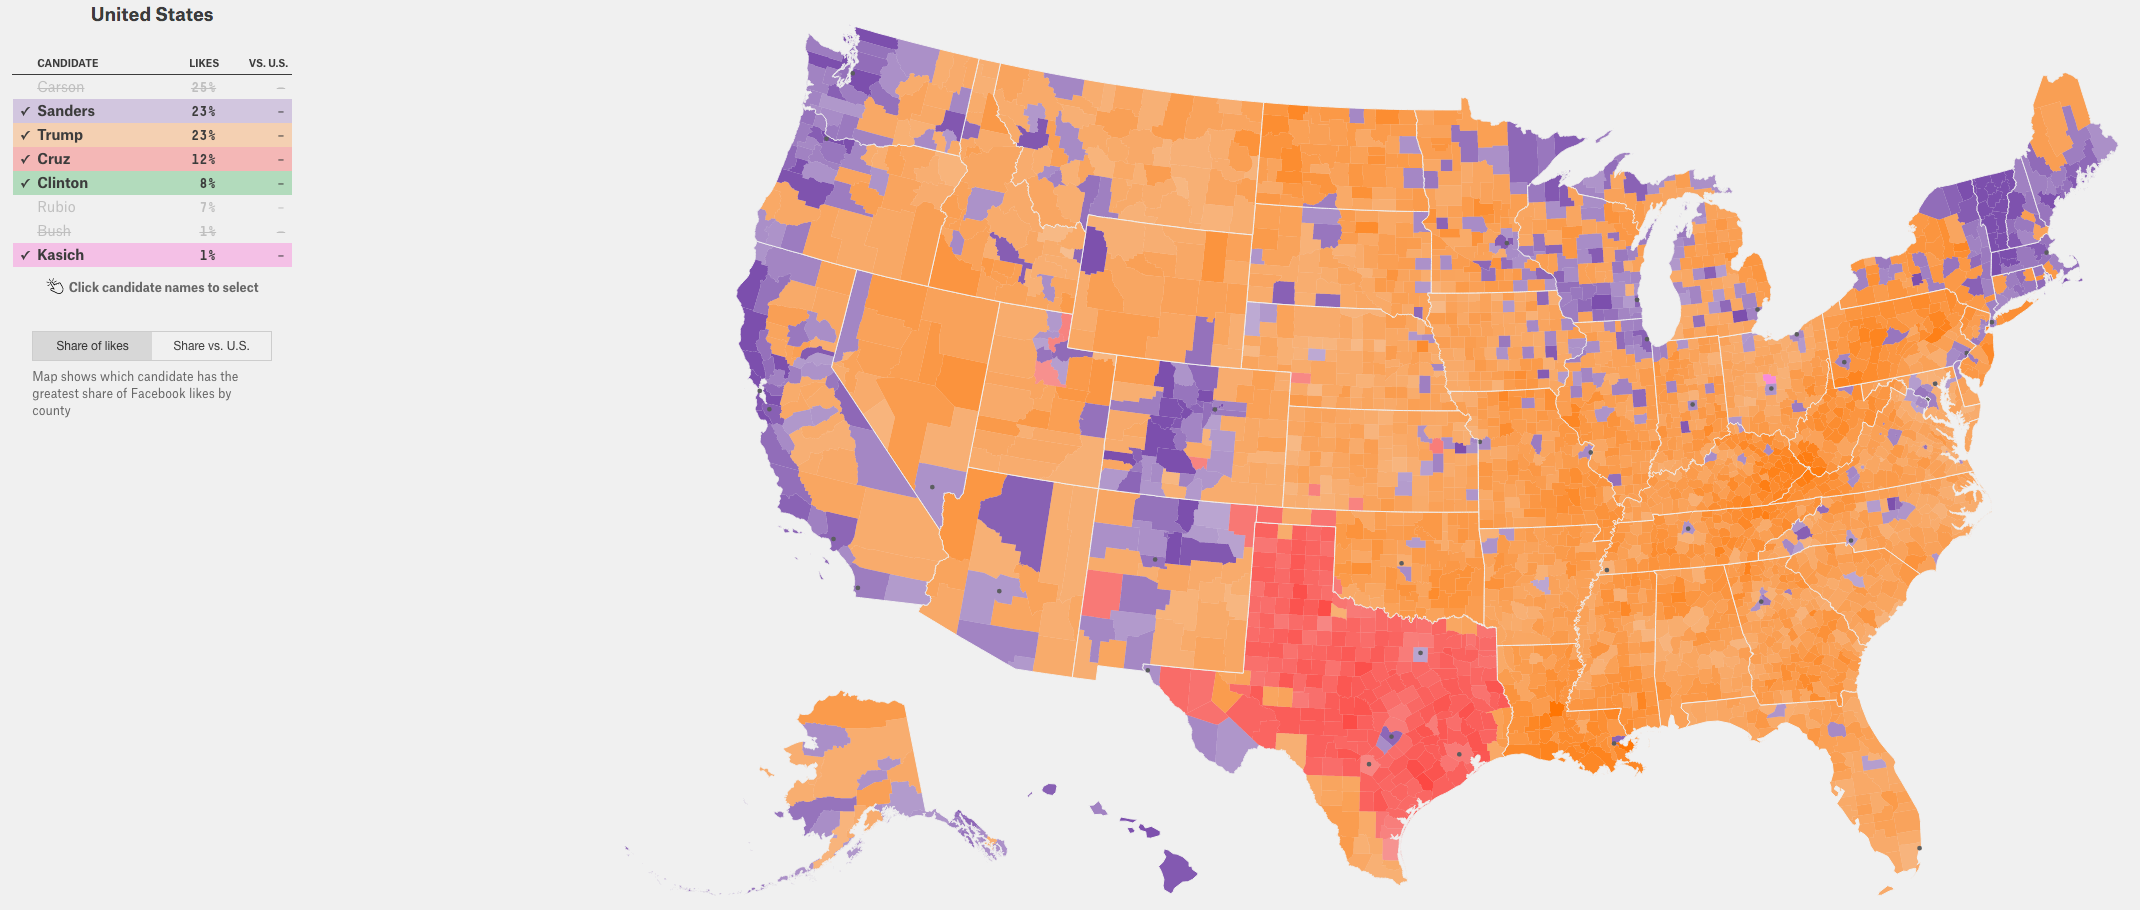
\includegraphics[scale=.14]{currentcandidate.png}
\end{center}
\end{frame}

\begin{frame}
\frametitle{Candidates and Social Media  \hfill 
\includegraphics[scale=.015]{images/likes.png}}
\begin{itemize}
\item Democratic Candidates
\end{itemize}
\begin{center}

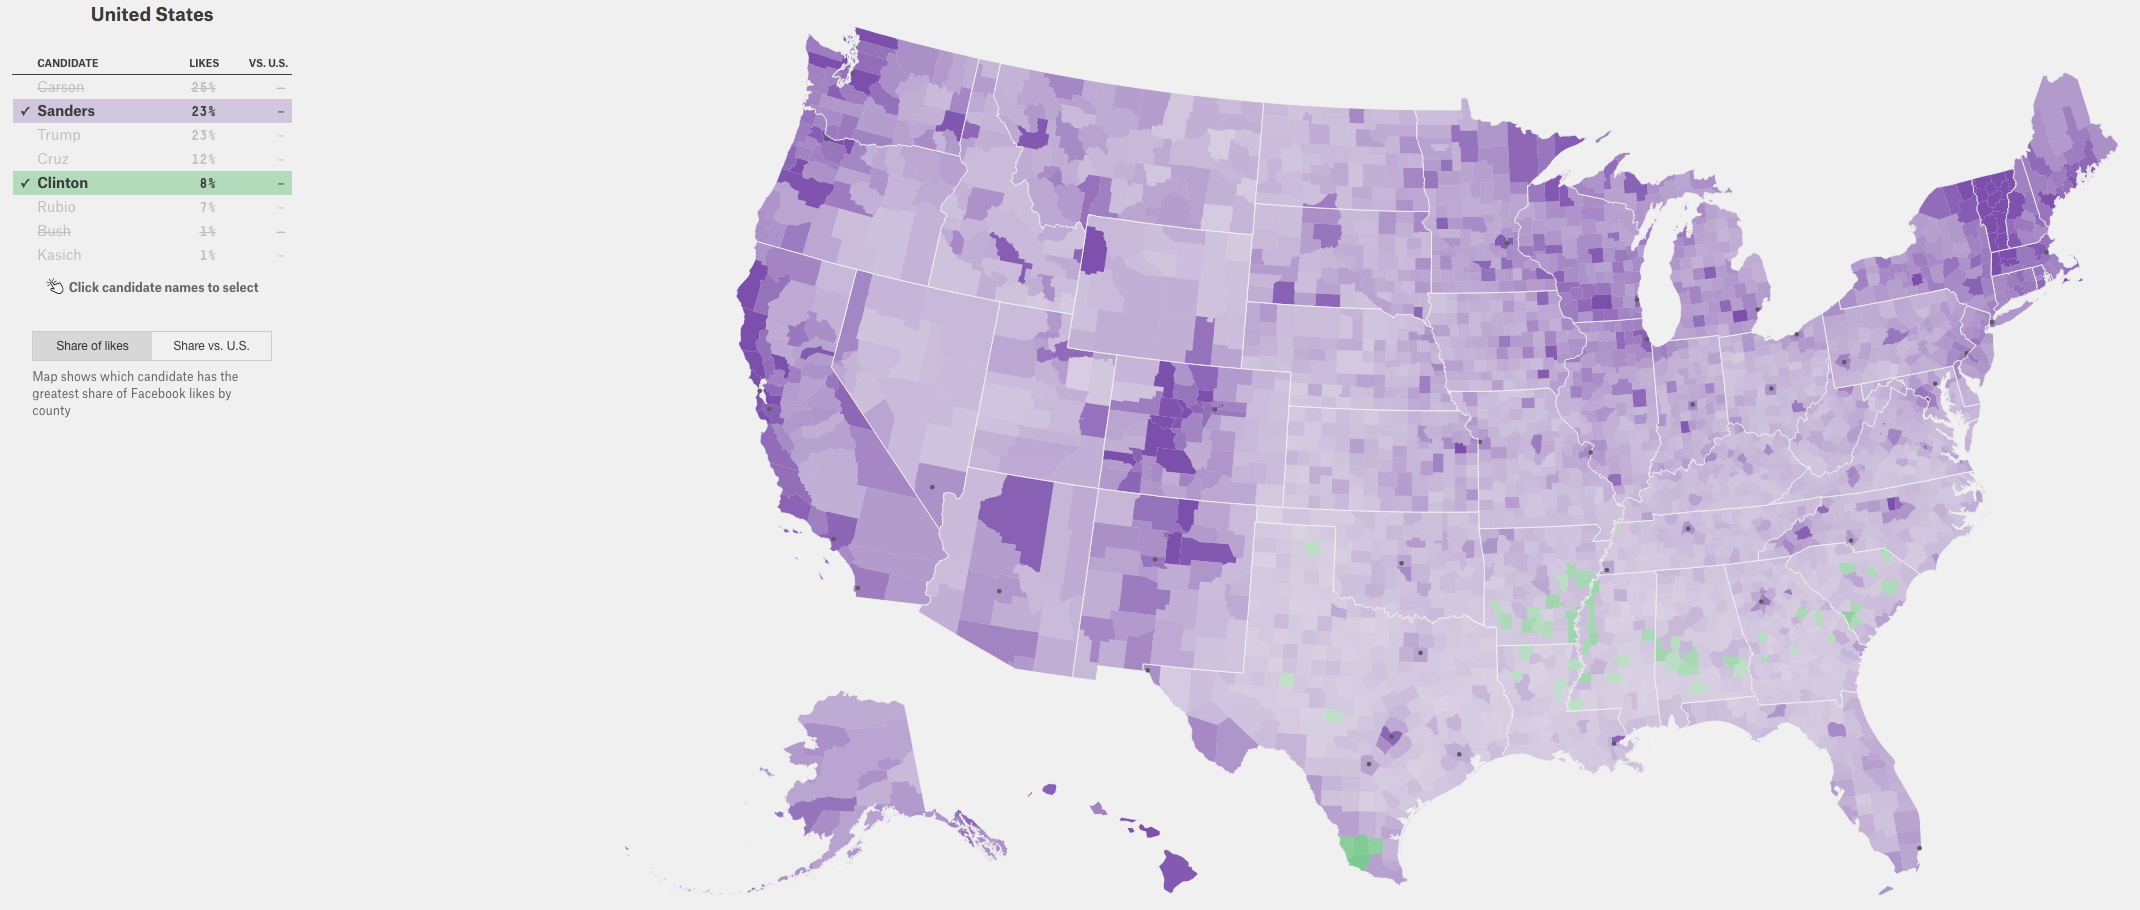
\includegraphics[scale=.14]{demmap.png}
\end{center}
\end{frame}

\begin{frame}
\frametitle{Candidates and Social Media  \hfill  
\includegraphics[scale=.015]{images/likes.png}}

\begin{itemize}
\item Republican Candidates 
\end{itemize}
\begin{center}

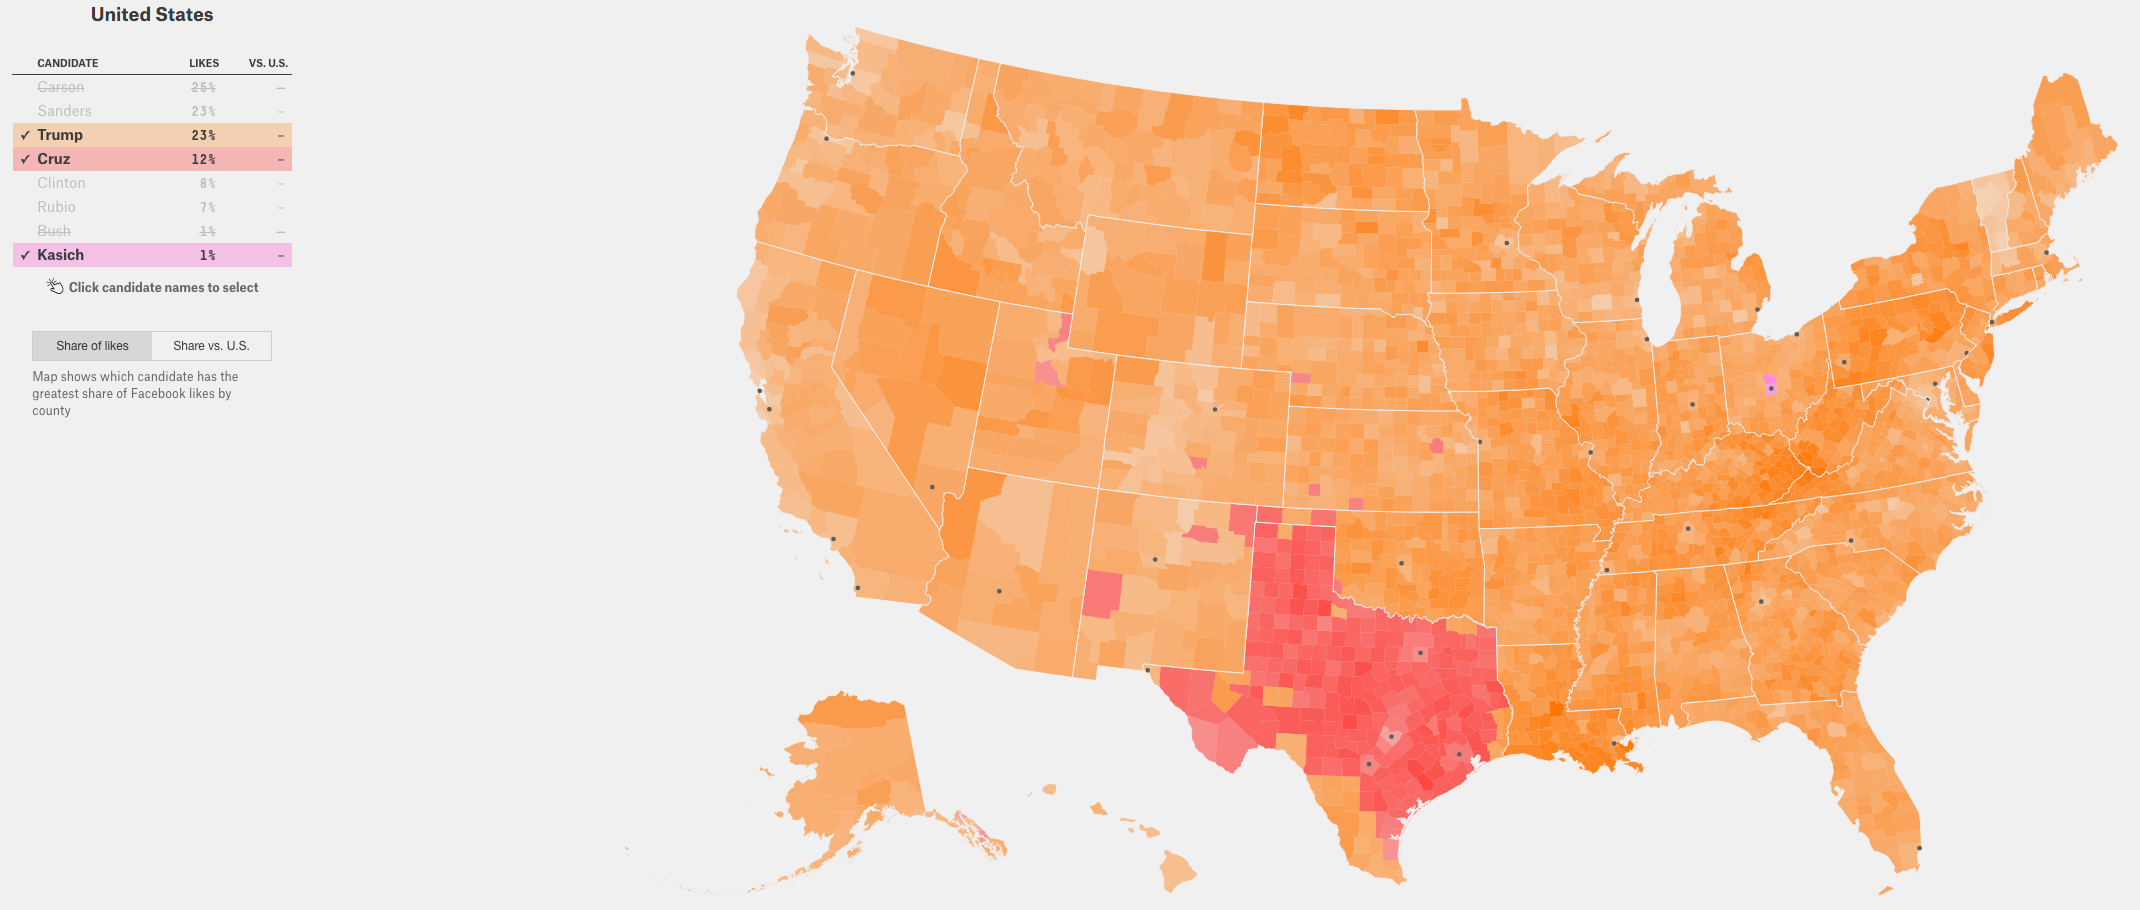
\includegraphics[scale=.14]{repmap.png}
\end{center}
\end{frame}


\begin{frame}
\section{Our Primary Predictions}
\frametitle{Natural Language Processing}
	\begin{itemize}
		\item Basic Idea
		\begin{itemize}
			\item Computers understanding language
		\end{itemize}
		\item Several Tasks in Natural Language Processing
		\begin{itemize}
			\item Question Answering
			\item Automatic Summarization
			\item Sentiment Analysis
		\end{itemize}
	\end{itemize}
\end{frame}



\begin{frame}
\frametitle{Popular Word Usage   \hfill 
\includegraphics[scale=.1]{twitterlogo.png}}
\begin{figure}[h!]
\subfloat[][]{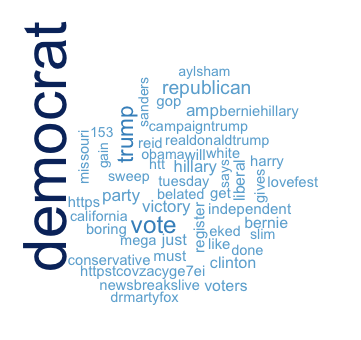
\includegraphics[scale=.38]{images/newwordclouddem}\label{Keyword ``Democrat}}
\hspace{1mm}
\subfloat[][]{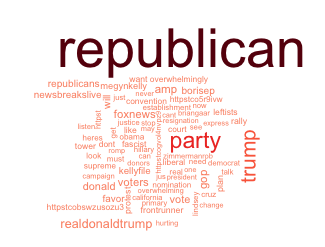
\includegraphics[scale = .4]{images/newwordcloudrep}\label{Keyword ``Republican}}
\caption{Word Clouds for Twitter Searches with Keywords ``Democrat'' and ``Republican''}
\end{figure}
\end{frame}

%\begin{frame}
%\frametitle{Popular Word Usage   \hfill 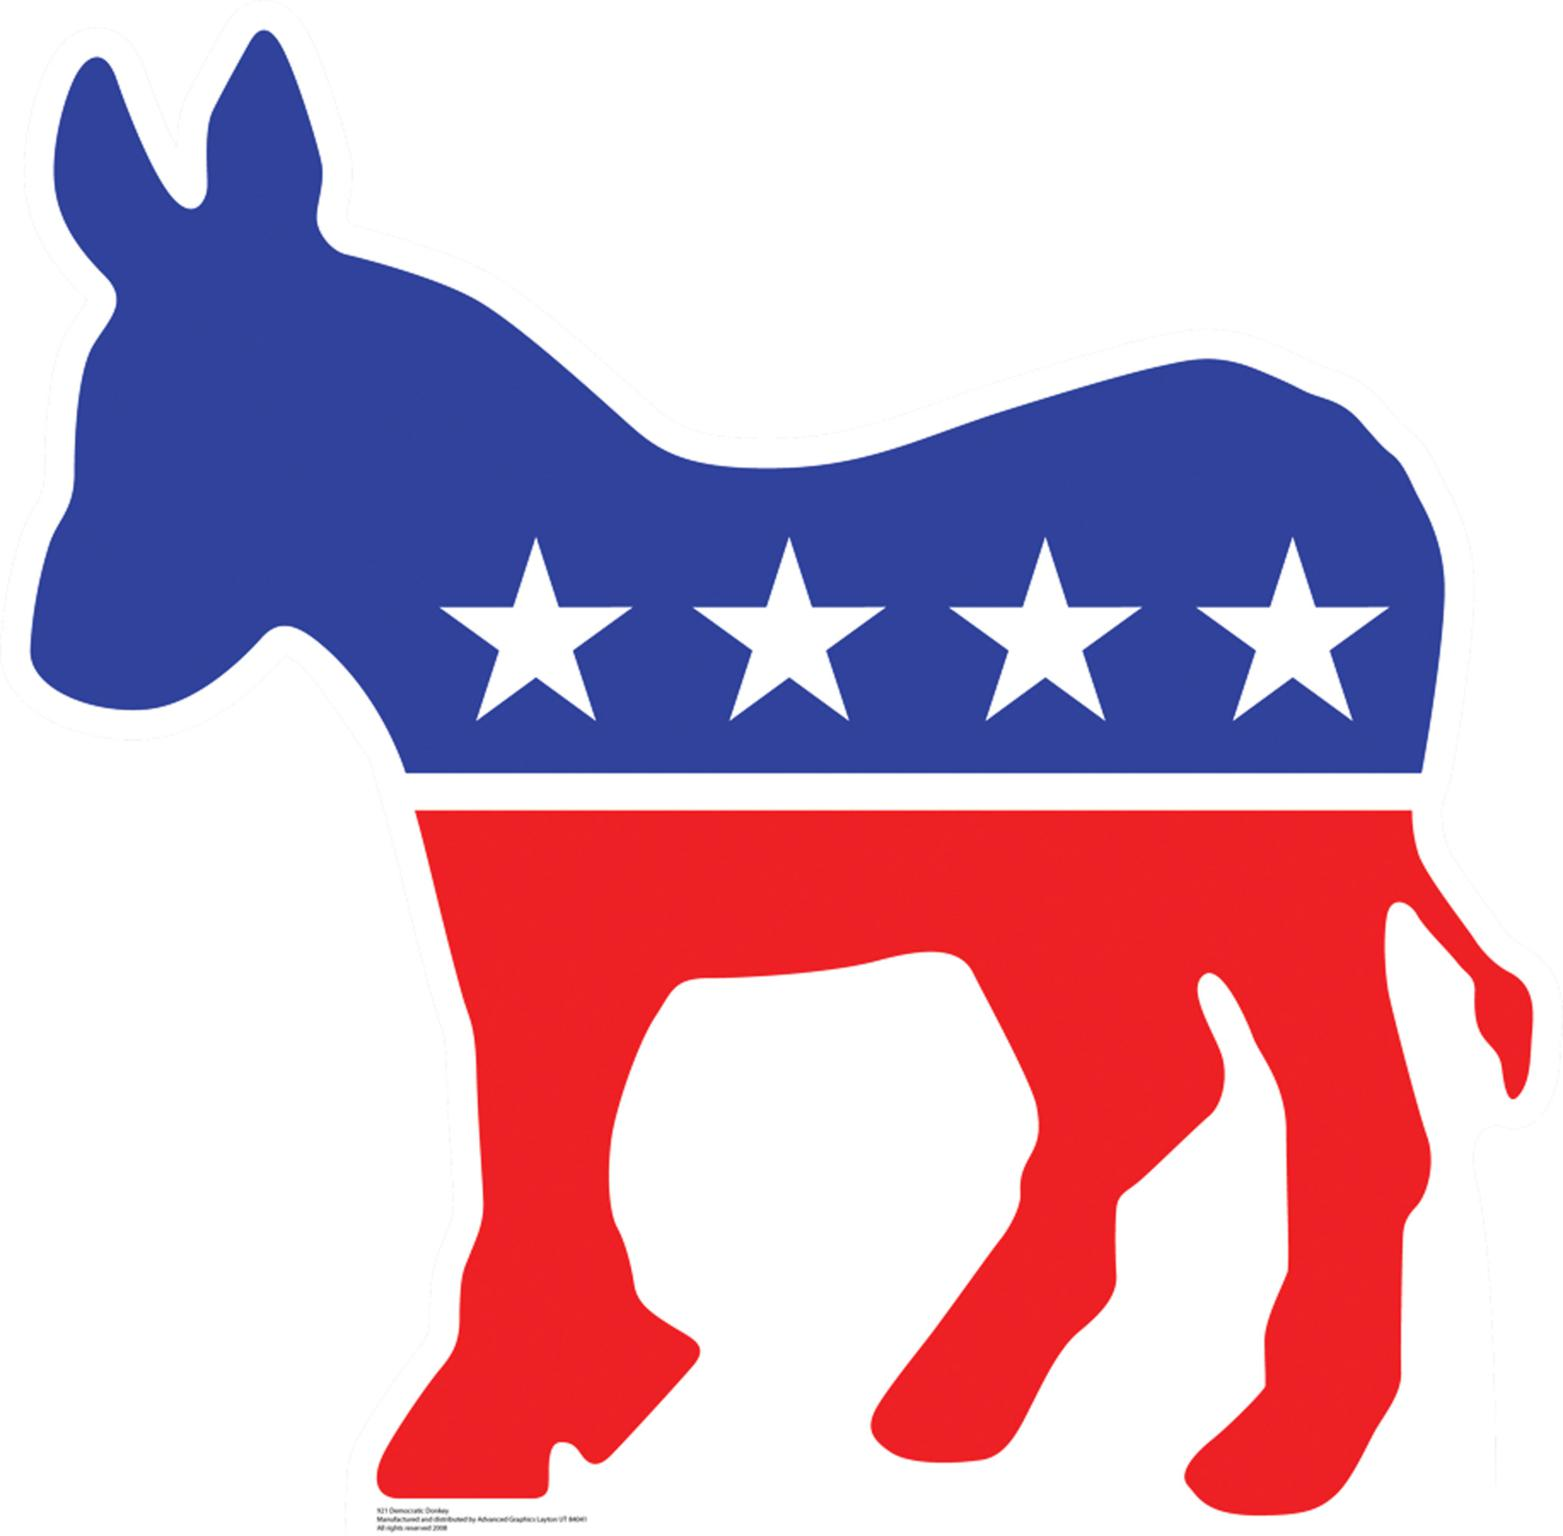
\includegraphics[scale=.01]{DemocraticLogo.jpg}}
%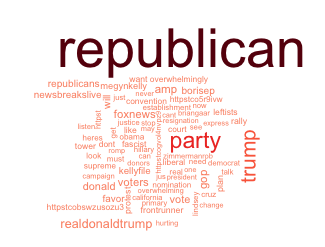
\includegraphics[scale=.55]{wcrepwithRT.png}	
%\end{frame}

\begin{frame}
\frametitle{Design of the Primary Prediction \\ \small In a Perfect World}
\subsection{Collecting Data}
\begin{itemize}
	\item Created a dataset with the names of all counties in US, their respective FIPS codes, and the recorded majority winners for each county 
	\begin{itemize}
	\item Unique identification number for each county in US
	\end{itemize}
	\item Found a dataset with area and centroid of each county in US
%	\begin{itemize}
%		\item Create a circle around centroid with radius equal to the $\sqrt{\text{Area}_{\text{county}}}$
%	\end{itemize}
	\item Search for tweets with specified keywords in every county of AZ, FL, IL, ID, MO, NC, OH, and UT
\begin{center}
\resizebox{.9\linewidth}{!}{
\begin{tabular}{|c|c|c|c|c|c|}
	\hline
	Candidates & Bernie Sanders & Hillary Clinton & Donald Trump & John Kasich & Ted Cruz \\
	\hline 
	Keywords & ``Bernie"  & ``I'm with Her" & ``Trump" & ``Kasich" & ``Cruz" \\
	&``Sanders" & "HillaryClinton" & ``Donald" & ``JohnKasich" & ``TedCruz \\
	& ``Feel The Bern'' & ``Hillary2016'' & ``Make America Great Again'' & ``Kasich2016'' & ``Trust Ted'' \\
	& ``Bernie2016'' & ``Clinton'' & ``Trump2016'' && ``TrustTed'' \\
	& & & ``DonaldTrump'' & & ``Cruz2016'' \\
	\hline
\end{tabular}}
	
\end{center}
	\item Merge results data frame with tweets data frame by FIPS code
	\end{itemize}
\end{frame}



%\begin{frame}
%\frametitle{Design of the Primary Prediction \\ \small In a Perfect World}
%\begin{itemize}
%\item Merge data frame with results with data frame of tweets by FIPS code
%	\begin{itemize}
%	\item Unique identification number for each county in US
%	\end{itemize}
%	\end{itemize}
%\end{frame}

\begin{frame}
\frametitle{Design of the Primary Prediction \\ \small In a Perfect World}
\subsection{Cleaning Tweets}
\large{An Example}\\
 Here is an original tweet from our collection: 
\begin{center}
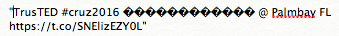
\includegraphics[scale=0.5]{uncleantweets3.png}
\end{center}
	\begin{itemize}
	\item Cleaning Tweets
	\begin{itemize}
		\item Remove punctuation
		\item Remove emojis
		\item Remove Stopwords
		\item Make everything lower case
	\end{itemize}
	\end{itemize}
\begin{center}
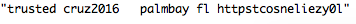
\includegraphics[scale=0.5]{CleanTweet.png}
\end{center}
\end{frame}

\begin{frame}
\frametitle{Design of the Primary Prediction \\ \small In a Perfect World}
\subsection{Models}
\begin{itemize}
	\item Create a Document-Term Matrix
	\begin{table}[h!]
	\resizebox{\linewidth}{!}{
	\begin{tabular}{|c|c|c|c|c|}
	\hline
	Doc Name & Term 1 & Term 2 & \dots & Term $n$ \\
	\hline
	Doc 1 & Freq(T1 in D1) & Freq(T2 in D1) & \dots & Freq(T$n$ in D1) \\
	\hline
	\vdots & & & & \\
	\hline
	Doc $m$ & Freq(T1 in D$m$) & Freq(T2 in D$m$) & \dots & Freq(T$n$ in D$m$) \\
	\hline
	\end{tabular}}
	\end{table}
	\item Attach labels to each tweet based on location of tweet
	\item Use machine learning algorithms to predict majority winners of each tweet's county
\end{itemize}
\end{frame}

\begin{frame}
\frametitle{Results \hfill 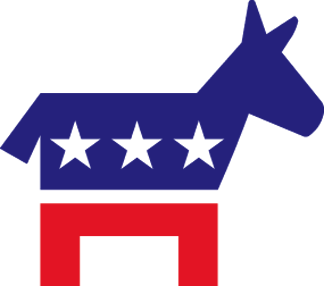
\includegraphics[scale=.12]{images/democraticlogo2.png}}
\section{Results}
\subsection{Democrats}
\begin{table}
\centering
\resizebox{.4\linewidth}{!}{
\begin{tabular}{cc|c|c|}
\cline{3-4}
 & & \multicolumn{2}{|c|}{Predicted} \\
 \cline{3-4}
 & & Bernie & Hillary \\
 \hline
 \multicolumn{1}{|c|}{\multirow{2}{*}{Actual}} & \multicolumn{1}{|c|}{Bernie} & 431 & 3332 \\
 \cline{2-4}
 \multicolumn{1}{|c|}{} & \multicolumn{1}{|c|}{Hillary} & 148 & 10212 \\
 \hline
\end{tabular}}
\caption{Support Vector Machine Confusion Matrix}
%This model has an accuracy of 75.35934\%
\end{table}
\begin{table}
\centering
\resizebox{.4\linewidth}{!}{
\begin{tabular}{cc|c|c|}
\cline{3-4}
 & & \multicolumn{2}{|c|}{Predicted} \\
 \cline{3-4}
 & & Bernie & Hillary \\
 \hline
 \multicolumn{1}{|c|}{\multirow{2}{*}{Actual}} & \multicolumn{1}{|c|}{Bernie} & 434 & 3329 \\
 \cline{2-4}
 \multicolumn{1}{|c|}{} & \multicolumn{1}{|c|}{Hillary} & 132 & 10228 \\
 \hline
\end{tabular}}
\caption{Neural Network Size 6 Confusion Matrix}
%Accuracy rate of 75.49388\%
\end{table}
\begin{table}
\centering
\resizebox{.4\linewidth}{!}{
\begin{tabular}{c|c}
 & Accuracy Rate \\
 \hline
Support Vector Machine & 75.35934\% \\
\hline
Neural Network & 75.49388\% \\
\end{tabular}}
\caption{Accuracy Rates of Both Models}
\end{table}

\end{frame}

\begin{frame}
\frametitle{Results \hfill 
\includegraphics[scale=.1]{republicanlogo.png}}
\subsection{Republicans}
\begin{figure}[h!]
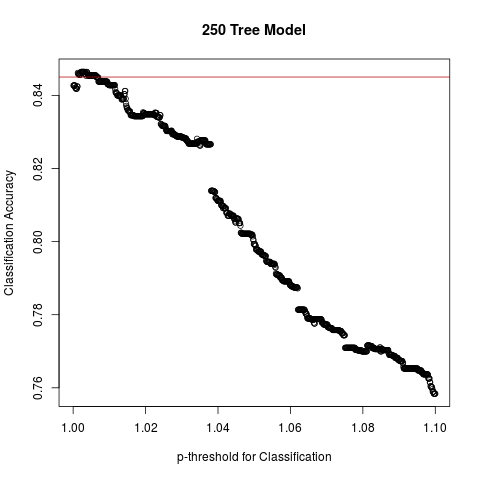
\includegraphics[scale = 0.2]{RFmodelaccuracy250.png}
\caption{A plot of classification accuracy versus probability threshold for Random Forest Model}
\end{figure}
\begin{table}
\centering
\resizebox{.4\linewidth}{!}{
\begin{tabular}{cc|c|c|}
\cline{3-4}
 & & \multicolumn{2}{|c|}{Predicted} \\
 \cline{3-4}
 & & Trump & Not Trump \\
 \hline
 \multicolumn{1}{|c|}{\multirow{2}{*}{Actual}} & \multicolumn{1}{|c|}{Trump} & 9517 & 42 \\
 \cline{2-4}
 \multicolumn{1}{|c|}{} & \multicolumn{1}{|c|}{Not Trump} & 1695 & 58 \\
 \hline
\end{tabular}}
\caption{Random Forest with 250 Trees Confusion Matrix.  Has an accuracy of 84.644625\%}
%Accuracy rate of 75.49388\%
\end{table}
\end{frame}

\begin{frame}
\frametitle{Limitations with Social Media \hfill \hfill 
\includegraphics[scale=.1]{twitterlogo.png}}
\section{Limitations}
\begin{itemize}
	\item Class imbalance - Trump is winning many more precincts than other Republican candidates
	\item Majority of Sanders supporters are younger and more likely to use Twitter (estimated at 88\% by Pew Research Center)
	\item According to the Pew Research Center, only 23\% of Americans use Twitter
	\item Twitter says that $<$ 5\% of all tweets are georeferenced
	\item Can only get tweets up to a week prior of collection time
	\item Could not find a comprehensive list of counties and results
	
\end{itemize}

\end{frame}

\begin{frame}
\frametitle{Future Work}
\section{Future Work}
\begin{itemize}
\item Continue to update our models for each Primary
\item Improve our models to account for other geographic differences
\item Use debate transcripts to predict partiality of media networks using online articles 
\item Extend current models to predict outcome of presidential election in November
\end{itemize}
\end{frame}

\begin{frame}
\frametitle{References}
\section{References}
\small{We'd like to thank the Office of Student Research and Creative Activity at Tarleton State University}
\begin{center}

\includegraphics[scale=.10]{images/thank-you}
\end{center}
\tiny
\noindent Benyamin, Dan.``A Gentle Introduction to Random Forests, Ensembles, and Performance Metrics in a \\
\hspace{1cm}Commercial System - Blog \& Press''  \textit{Citizen and Net.} N.p., 09 Nov. 2012. \\
\hspace{1cm}Web. 28 Mar. 2016. \\
Phillips, Winfred.  ``Introduction to Natural Language Processing.'' \textit{Consortium on Cognitive Science} \\
\hspace{1cm}\textit{Instruction.} The MIND Project, 2006.  Web.  16 Mar 2016. \\
Raine, Lee. ``Social Media and Voting." \textit{Pew Research Center Internet} \textit{Science Tech RSS.} Pew Charitable \\
\hspace{1cm}Trusts, 05 Nov. 2012. Web. 28 Mar. 2016.
Weston, Jason. ``Support Vector Machines (and Statistical Learning Theory)." ComputerScience4701. \\
\hspace{1cm}Columbia University, New York. \textit{Columbia University}. Web. 28 Mar. 2016.\\
``FiveThirtyEight.'' \textit{FiveThirtyEight.} Nate Silver, n.d. Web.  28 Mar 2016. \\
``2016 Primary Election Results: President Live Map by State, Real-Time Voting Updates'' \textit{Election Hub.} \\ 
\hspace{1cm}Politico LLC, 27 Mar. 2016.  Web.  28 Mar. 2016. \\
\end{frame}





\end{document}